% !TEX program = lualatex

%The Aspectration can be 4:3 (43) and 16:9 (169)
\documentclass[12pt, aspectratio=169, usepdftitle=false]{beamer}
% \documentclass[12pt, aspectratio=169, usepdftitle=false, handout]{beamer}

\usepackage[ngerman]{babel}
\usepackage{marvosym}
\usepackage{pifont}
\usepackage{pgfpages} 
\usepackage{ifthen}
\usepackage{ragged2e}

\usepackage{ubo_tex_beamer/uni-template}
\apptocmd{\frame}{}{\justifying}{} % Allow optional arguments after frame.
% SET TITLE
%----------------------------
\MainTitle{Vertiefungskurs Python}
\SubTitle{\ }

% SET AUTHOR
%----------------------------
\AuthorName{Chris Geron}
\AuthorEmail{s6chgero@uni-bonn.de}
\AuthorInformation{Institut für Informatik}

% SET EVENT-INFORMATION
%----------------------------
\Eventname{Vertiefungskurs Python}
\City{Universität Bonn}
\Date{SoSe 2023}

% Drucke Gitversion
\renewcommand{\printgitversion}{true}
% Drucke Dateinamen
\renewcommand{\printfilename}{true}


% custom packages

\lstset{ backgroundcolor=\color{colororange!5} }

% Include pictures made in inkscape:
\newcommand{\inputhack}{\input}        % Rename \input, so that a very simple awk-skript can merge all tex-files.
\graphicspath{{images/}}               % Set path of the pictures. This is used by the pdf_tex-files generated by inkscape.
\newcommand{\inkpic}[2][\columnwidth]{%
  \def\svgwidth{#1}%
  \inputhack{images/#2.pdf_tex}%
}

\newcommand{\tb}[1]{\textbf{#1}}
\newcommand{\extrainfo}{\begin{textblock}{1}(14.4,.3)\hfuzz=\maxdimen
\includegraphics[width=1.3cm]{images/extra_info.pdf}\end{textblock}}
\newtheorem{defi}{}


\usepackage{textpos}
\setlength{\TPHorizModule}{1cm}
\setlength{\TPVertModule}{1cm}

\newcommand\crule[1][black]{\textcolor{#1}{\rule{2cm}{2cm}}}
\newcommand{\arroworange}{\color{colororange}\Large\MVRightarrow}
\newcommand{\arrowyellow}{\color{coloryellow}\Large\MVRightarrow}
\newcommand{\arrowblue}{\color{colorblue}\Large\MVRightarrow}

\newcommand{\cmark}{\ding{51}}%
\newcommand{\xmark}{\ding{55}}%


\newcommand{\mcO}{\mathcal{O}}


\newcommand{\umlkeyword}[1]{{\color{black}\guillemotleft{}\lpl{#1}\guillemotright{}}}


\newcommand{\shrug}[1][]{%
\begin{tikzpicture}[baseline,x=0.8\ht\strutbox,y=0.8\ht\strutbox,line width=0.125ex,#1]
\def\arm{(-2.5,0.95) to (-2,0.95) (-1.9,1) to (-1.5,0) (-1.35,0) to (-0.8,0)};
\draw \arm;
\draw[xscale=-1] \arm;
\def\headpart{(0.6,0) arc[start angle=-40, end angle=40,x radius=0.6,y radius=0.8]};
\draw \headpart;
\draw[xscale=-1] \headpart;
\def\eye{(-0.075,0.15) .. controls (0.02,0) .. (0.075,-0.15)};
\draw[shift={(-0.3,0.8)}] \eye;
\draw[shift={(0,0.85)}] \eye;
% draw mouth
\draw (-0.1,0.2) to [out=15,in=-100] (0.4,0.95); 
\end{tikzpicture}}


\usepackage{forest}
\forestset{
  default preamble={
    for tree={
      circle,
      draw,
      thick,
      color=black,
      fill=colororange!25,
      text=black,
      minimum size=1.5ex,
      edge+={draw=black, thick},
    },
    delay={
      where content={}{% just the empty nodes
        phantom,
      }{},
    },
  }
}

\tikzset{
  node/.style={
    text=black,
    draw=black,
  },
  tri/.style={
    draw=black,
    isosceles triangle,
    isosceles triangle apex angle=22,
    shape border rotate=90,
    inner sep=0.1pt,
    minimum width=0.5cm,
  }
}

% UML Diagramme
\let\attribute\relax % Workaround needed for old pgf-umlcd-packages
\usepackage[simplified]{pgf-umlcd}
\usetikzlibrary{arrows, arrows.meta}
\providecommand{\umltextcolor}{}
\providecommand{\umlfillcolor}{}
\providecommand{\umldrawcolor}{}
\renewcommand{\umltextcolor}{colorblue}
\renewcommand{\umlfillcolor}{coloryellow!20}
\renewcommand{\umldrawcolor}{coloryellow}

\tikzstyle{classdiag} = [
  every node/.style = {font=\footnotesize}
]

\tikzset{
  template parameter/.style={
    append after command={
      node [draw, densely dashed, umlcolor, font=\ttfamily]
        at (\tikzlastnode.north east)
        {#1}
    }
  }
}

\tikzstyle{umlnode} = [
  font=\footnotesize\bfseries,
  draw=coloryellow,
  fill=coloryellow!20,
  text width=3.5cm,
  align=center,
  anchor=north west
]

\tikzstyle{umlarrow} = [
  thick,
  draw=coloryellow
]

\newcommand{\todo}[1]{\textbf{\color{red}\ #1 \ }}

\newcommand{\framecardfragen}{
  \framecardorange{
    \utext{Haben Sie Fragen?}
  }
}


% Socket und Plug
\makeatletter

\pgfdeclareshape{rotsocket}
{
  \inheritsavedanchors[from=circle] % this is nearly a circle
  \inheritanchorborder[from=circle]
  \inheritanchor[from=circle]{north}
  \inheritanchor[from=circle]{north west}
  \inheritanchor[from=circle]{north east}
  \inheritanchor[from=circle]{center}
  \inheritanchor[from=circle]{west}
  \inheritanchor[from=circle]{east}
  \inheritanchor[from=circle]{mid}
  \inheritanchor[from=circle]{mid west}
  \inheritanchor[from=circle]{mid east}
  \inheritanchor[from=circle]{base}
  \inheritanchor[from=circle]{base west}
  \inheritanchor[from=circle]{base east}
  \inheritanchor[from=circle]{south}
  \inheritanchor[from=circle]{south west}
  \inheritanchor[from=circle]{south east}
%   \inheritbackgroundpath[from=circle]
  \foregroundpath{
    \centerpoint%
    \pgf@xc=\pgf@x%                                                                                                                   \pgf@xc = x value of centerpoint
    \pgf@yc=\pgf@y%                                                                                                                   \pgf@yc = y value of centerpoint
    \pgfutil@tempdima=\radius%                                                                                              \pgfutil@tempdima = radius
    \pgfmathsetlength{\pgf@xb}{\pgfkeysvalueof{/pgf/outer xsep}}%                                                                     \pgf@xb = outer xsep
    \pgfmathsetlength{\pgf@yb}{\pgfkeysvalueof{/pgf/outer ysep}}%                                                                     \pgf@yb = outer ysep
    \pgfmathsetmacro{\pgf@socket@rotate}{\pgfkeysvalueof{/tikz/socket rotate}}%                                            \pgf@socket@rotate = socket rotate
    \ifdim\pgf@xb<\pgf@yb%
      \advance\pgfutil@tempdima by-\pgf@yb%
    \else%
      \advance\pgfutil@tempdima by-\pgf@xb%
    \fi%
    % Background color
    \pgfpathmoveto{\pgfpointadd{\pgfqpoint{\pgf@xc}{\pgf@yc}}{\pgfqpoint{-0.65\pgfutil@tempdima}{ 0.5\pgfutil@tempdima}}}
    \pgfpathlineto{\pgfpointadd{\pgfqpoint{\pgf@xc}{\pgf@yc}}{\pgfqpoint{-0.86602540378\pgfutil@tempdima}{ 0.5\pgfutil@tempdima}}}
    \pgfpatharc{150}{210}{\pgfutil@tempdima}
    \pgfpathlineto{\pgfpointadd{\pgfqpoint{\pgf@xc}{\pgf@yc}}{\pgfqpoint{-0.65\pgfutil@tempdima}{-0.5\pgfutil@tempdima}}}
    \pgfpathlineto{\pgfpointadd{\pgfqpoint{\pgf@xc}{\pgf@yc}}{\pgfqpoint{-0.20\pgfutil@tempdima}{-0.7\pgfutil@tempdima}}}
    \pgfpathlineto{\pgfpointadd{\pgfqpoint{\pgf@xc}{\pgf@yc}}{\pgfqpoint{ 0.60\pgfutil@tempdima}{-0.7\pgfutil@tempdima}}}
    \pgfpathlineto{\pgfpointadd{\pgfqpoint{\pgf@xc}{\pgf@yc}}{\pgfqpoint{ 0.60\pgfutil@tempdima}{ 0.7\pgfutil@tempdima}}}
    \pgfpathlineto{\pgfpointadd{\pgfqpoint{\pgf@xc}{\pgf@yc}}{\pgfqpoint{-0.20\pgfutil@tempdima}{ 0.7\pgfutil@tempdima}}}
    \pgfpathclose
    \pgfsetfillcolor{gray!15}
    \pgfusepath{fill}
    
    % Stroke
    \pgfpathmoveto{\pgfpointadd{\pgfqpoint{\pgf@xc}{\pgf@yc}}{\pgfqpoint{-0.65\pgfutil@tempdima}{ 0.5\pgfutil@tempdima}}}
    \pgfpathlineto{\pgfpointadd{\pgfqpoint{\pgf@xc}{\pgf@yc}}{\pgfqpoint{-0.80\pgfutil@tempdima}{ 0.5\pgfutil@tempdima}}}
    \pgfpathlineto{\pgfpointadd{\pgfqpoint{\pgf@xc}{\pgf@yc}}{\pgfqpoint{-0.86602540378\pgfutil@tempdima}{ 0.5\pgfutil@tempdima}}}
    \pgfpatharc{150}{210}{\pgfutil@tempdima}
    \pgfpathlineto{\pgfpointadd{\pgfqpoint{\pgf@xc}{\pgf@yc}}{\pgfqpoint{-0.80\pgfutil@tempdima}{-0.5\pgfutil@tempdima}}}
    \pgfpathlineto{\pgfpointadd{\pgfqpoint{\pgf@xc}{\pgf@yc}}{\pgfqpoint{-0.80\pgfutil@tempdima}{ 0.5\pgfutil@tempdima}}}
    
    \pgfpathmoveto{\pgfpointadd{\pgfqpoint{\pgf@xc}{\pgf@yc}}{\pgfqpoint{-0.80\pgfutil@tempdima}{-0.5\pgfutil@tempdima}}}
    \pgfpathlineto{\pgfpointadd{\pgfqpoint{\pgf@xc}{\pgf@yc}}{\pgfqpoint{-0.65\pgfutil@tempdima}{-0.5\pgfutil@tempdima}}}
    \pgfpathlineto{\pgfpointadd{\pgfqpoint{\pgf@xc}{\pgf@yc}}{\pgfqpoint{-0.65\pgfutil@tempdima}{ 0.5\pgfutil@tempdima}}}
    \pgfpathlineto{\pgfpointadd{\pgfqpoint{\pgf@xc}{\pgf@yc}}{\pgfqpoint{-0.20\pgfutil@tempdima}{ 0.7\pgfutil@tempdima}}}
    \pgfpathlineto{\pgfpointadd{\pgfqpoint{\pgf@xc}{\pgf@yc}}{\pgfqpoint{ 0.60\pgfutil@tempdima}{ 0.7\pgfutil@tempdima}}}
    \pgfpathlineto{\pgfpointadd{\pgfqpoint{\pgf@xc}{\pgf@yc}}{\pgfqpoint{ 0.60\pgfutil@tempdima}{-0.7\pgfutil@tempdima}}}
    \pgfpathlineto{\pgfpointadd{\pgfqpoint{\pgf@xc}{\pgf@yc}}{\pgfqpoint{-0.20\pgfutil@tempdima}{-0.7\pgfutil@tempdima}}}
    \pgfpathlineto{\pgfpointadd{\pgfqpoint{\pgf@xc}{\pgf@yc}}{\pgfqpoint{-0.65\pgfutil@tempdima}{-0.5\pgfutil@tempdima}}}
    
    \pgfpathmoveto{\pgfpointadd{\pgfqpoint{\pgf@xc}{\pgf@yc}}{\pgfqpoint{-0.55\pgfutil@tempdima}{-0.40\pgfutil@tempdima}}}
    \pgfpathlineto{\pgfpointadd{\pgfqpoint{\pgf@xc}{\pgf@yc}}{\pgfqpoint{-0.20\pgfutil@tempdima}{-0.55\pgfutil@tempdima}}}
    \pgfpathlineto{\pgfpointadd{\pgfqpoint{\pgf@xc}{\pgf@yc}}{\pgfqpoint{ 0.45\pgfutil@tempdima}{-0.55\pgfutil@tempdima}}}
    
    \pgfsetstrokecolor{black}
    \pgfusepath{stroke}
  }
}


\pgfdeclareshape{rotplug}
{
  \inheritsavedanchors[from=circle] % this is nearly a circle
  \inheritanchorborder[from=circle]
  \inheritanchor[from=circle]{north}
  \inheritanchor[from=circle]{north west}
  \inheritanchor[from=circle]{north east}
  \inheritanchor[from=circle]{center}
  \inheritanchor[from=circle]{west}
  \inheritanchor[from=circle]{east}
  \inheritanchor[from=circle]{mid}
  \inheritanchor[from=circle]{mid west}
  \inheritanchor[from=circle]{mid east}
  \inheritanchor[from=circle]{base}
  \inheritanchor[from=circle]{base west}
  \inheritanchor[from=circle]{base east}
  \inheritanchor[from=circle]{south}
  \inheritanchor[from=circle]{south west}
  \inheritanchor[from=circle]{south east}
%   \inheritbackgroundpath[from=circle]
  \foregroundpath{
    \centerpoint%
    \pgf@xc=\pgf@x%                                                                                                                   \pgf@xc = x value of centerpoint
    \pgf@yc=\pgf@y%                                                                                                                   \pgf@yc = y value of centerpoint
    \pgfutil@tempdima=\radius%                                                                                              \pgfutil@tempdima = radius
    \pgfmathsetlength{\pgf@xb}{\pgfkeysvalueof{/pgf/outer xsep}}%                                                                     \pgf@xb = outer xsep
    \pgfmathsetlength{\pgf@yb}{\pgfkeysvalueof{/pgf/outer ysep}}%                                                                     \pgf@yb = outer ysep
    \pgfmathsetmacro{\pgf@plug@rotate}{\pgfkeysvalueof{/tikz/plug rotate}}%                                                  \pgf@plug@rotate = plug rotate
    \ifdim\pgf@xb<\pgf@yb%
      \advance\pgfutil@tempdima by-\pgf@yb%
    \else%
      \advance\pgfutil@tempdima by-\pgf@xb%
    \fi%
    % Background color
    \pgfpathmoveto{\pgfpointadd{\pgfqpoint{\pgf@xc}{\pgf@yc}}{\pgfqpoint{-0.65\pgfutil@tempdima}{ 0.5\pgfutil@tempdima}}}
    \pgfpathlineto{\pgfpointadd{\pgfqpoint{\pgf@xc}{\pgf@yc}}{\pgfqpoint{-0.86602540378\pgfutil@tempdima}{ 0.5\pgfutil@tempdima}}}
    \pgfpatharc{150}{210}{\pgfutil@tempdima}
    \pgfpathlineto{\pgfpointadd{\pgfqpoint{\pgf@xc}{\pgf@yc}}{\pgfqpoint{-0.65\pgfutil@tempdima}{-0.5\pgfutil@tempdima}}}
    \pgfpathlineto{\pgfpointadd{\pgfqpoint{\pgf@xc}{\pgf@yc}}{\pgfqpoint{-0.20\pgfutil@tempdima}{-0.7\pgfutil@tempdima}}}
    \pgfpathlineto{\pgfpointadd{\pgfqpoint{\pgf@xc}{\pgf@yc}}{\pgfqpoint{ 0.60\pgfutil@tempdima}{-0.7\pgfutil@tempdima}}}
    \pgfpathlineto{\pgfpointadd{\pgfqpoint{\pgf@xc}{\pgf@yc}}{\pgfqpoint{ 0.60\pgfutil@tempdima}{ 0.7\pgfutil@tempdima}}}
    \pgfpathlineto{\pgfpointadd{\pgfqpoint{\pgf@xc}{\pgf@yc}}{\pgfqpoint{-0.20\pgfutil@tempdima}{ 0.7\pgfutil@tempdima}}}
    \pgfpathclose
    \pgfsetfillcolor{gray!15}
    \pgfusepath{fill}
    
    \pgfpathmoveto{\pgfpointadd{\pgfqpoint{\pgf@xc}{\pgf@yc}}{\pgfqpoint{ 0.60\pgfutil@tempdima}{ 0.50\pgfutil@tempdima}}}
    \pgfpathlineto{\pgfpointadd{\pgfqpoint{\pgf@xc}{\pgf@yc}}{\pgfqpoint{ 1.30\pgfutil@tempdima}{ 0.50\pgfutil@tempdima}}}
    \pgfpathlineto{\pgfpointadd{\pgfqpoint{\pgf@xc}{\pgf@yc}}{\pgfqpoint{ 1.45\pgfutil@tempdima}{ 0.45\pgfutil@tempdima}}}
    \pgfpathlineto{\pgfpointadd{\pgfqpoint{\pgf@xc}{\pgf@yc}}{\pgfqpoint{ 1.45\pgfutil@tempdima}{ 0.35\pgfutil@tempdima}}}
    \pgfpathlineto{\pgfpointadd{\pgfqpoint{\pgf@xc}{\pgf@yc}}{\pgfqpoint{ 1.30\pgfutil@tempdima}{ 0.30\pgfutil@tempdima}}}
    \pgfpathlineto{\pgfpointadd{\pgfqpoint{\pgf@xc}{\pgf@yc}}{\pgfqpoint{ 0.60\pgfutil@tempdima}{ 0.30\pgfutil@tempdima}}}
    \pgfpathclose
    
    \pgfpathmoveto{\pgfpointadd{\pgfqpoint{\pgf@xc}{\pgf@yc}}{\pgfqpoint{ 0.60\pgfutil@tempdima}{-0.50\pgfutil@tempdima}}}
    \pgfpathlineto{\pgfpointadd{\pgfqpoint{\pgf@xc}{\pgf@yc}}{\pgfqpoint{ 1.30\pgfutil@tempdima}{-0.50\pgfutil@tempdima}}}
    \pgfpathlineto{\pgfpointadd{\pgfqpoint{\pgf@xc}{\pgf@yc}}{\pgfqpoint{ 1.45\pgfutil@tempdima}{-0.45\pgfutil@tempdima}}}
    \pgfpathlineto{\pgfpointadd{\pgfqpoint{\pgf@xc}{\pgf@yc}}{\pgfqpoint{ 1.45\pgfutil@tempdima}{-0.35\pgfutil@tempdima}}}
    \pgfpathlineto{\pgfpointadd{\pgfqpoint{\pgf@xc}{\pgf@yc}}{\pgfqpoint{ 1.30\pgfutil@tempdima}{-0.30\pgfutil@tempdima}}}
    \pgfpathlineto{\pgfpointadd{\pgfqpoint{\pgf@xc}{\pgf@yc}}{\pgfqpoint{ 0.60\pgfutil@tempdima}{-0.30\pgfutil@tempdima}}}
    \pgfpathclose
    \pgfsetfillcolor{coloryellow!30}
    \pgfusepath{fill}
    
    % Foreground stroke
    \pgfpathmoveto{\pgfpointadd{\pgfqpoint{\pgf@xc}{\pgf@yc}}{\pgfqpoint{-0.65\pgfutil@tempdima}{ 0.5\pgfutil@tempdima}}}
    \pgfpathlineto{\pgfpointadd{\pgfqpoint{\pgf@xc}{\pgf@yc}}{\pgfqpoint{-0.80\pgfutil@tempdima}{ 0.5\pgfutil@tempdima}}}
    \pgfpathlineto{\pgfpointadd{\pgfqpoint{\pgf@xc}{\pgf@yc}}{\pgfqpoint{-0.86602540378\pgfutil@tempdima}{ 0.5\pgfutil@tempdima}}}
    \pgfpatharc{150}{210}{\pgfutil@tempdima}
    \pgfpathlineto{\pgfpointadd{\pgfqpoint{\pgf@xc}{\pgf@yc}}{\pgfqpoint{-0.80\pgfutil@tempdima}{-0.5\pgfutil@tempdima}}}
    \pgfpathlineto{\pgfpointadd{\pgfqpoint{\pgf@xc}{\pgf@yc}}{\pgfqpoint{-0.80\pgfutil@tempdima}{ 0.5\pgfutil@tempdima}}}
    
    \pgfpathmoveto{\pgfpointadd{\pgfqpoint{\pgf@xc}{\pgf@yc}}{\pgfqpoint{-0.80\pgfutil@tempdima}{-0.5\pgfutil@tempdima}}}
    \pgfpathlineto{\pgfpointadd{\pgfqpoint{\pgf@xc}{\pgf@yc}}{\pgfqpoint{-0.65\pgfutil@tempdima}{-0.5\pgfutil@tempdima}}}
    \pgfpathlineto{\pgfpointadd{\pgfqpoint{\pgf@xc}{\pgf@yc}}{\pgfqpoint{-0.65\pgfutil@tempdima}{ 0.5\pgfutil@tempdima}}}
    \pgfpathlineto{\pgfpointadd{\pgfqpoint{\pgf@xc}{\pgf@yc}}{\pgfqpoint{-0.20\pgfutil@tempdima}{ 0.7\pgfutil@tempdima}}}
    \pgfpathlineto{\pgfpointadd{\pgfqpoint{\pgf@xc}{\pgf@yc}}{\pgfqpoint{ 0.60\pgfutil@tempdima}{ 0.7\pgfutil@tempdima}}}
    \pgfpathlineto{\pgfpointadd{\pgfqpoint{\pgf@xc}{\pgf@yc}}{\pgfqpoint{ 0.60\pgfutil@tempdima}{-0.7\pgfutil@tempdima}}}
    \pgfpathlineto{\pgfpointadd{\pgfqpoint{\pgf@xc}{\pgf@yc}}{\pgfqpoint{-0.20\pgfutil@tempdima}{-0.7\pgfutil@tempdima}}}
    \pgfpathlineto{\pgfpointadd{\pgfqpoint{\pgf@xc}{\pgf@yc}}{\pgfqpoint{-0.65\pgfutil@tempdima}{-0.5\pgfutil@tempdima}}}
    
    \pgfpathmoveto{\pgfpointadd{\pgfqpoint{\pgf@xc}{\pgf@yc}}{\pgfqpoint{ 0.60\pgfutil@tempdima}{ 0.50\pgfutil@tempdima}}}
    \pgfpathlineto{\pgfpointadd{\pgfqpoint{\pgf@xc}{\pgf@yc}}{\pgfqpoint{ 1.30\pgfutil@tempdima}{ 0.50\pgfutil@tempdima}}}
    \pgfpathlineto{\pgfpointadd{\pgfqpoint{\pgf@xc}{\pgf@yc}}{\pgfqpoint{ 1.45\pgfutil@tempdima}{ 0.45\pgfutil@tempdima}}}
    \pgfpathlineto{\pgfpointadd{\pgfqpoint{\pgf@xc}{\pgf@yc}}{\pgfqpoint{ 1.45\pgfutil@tempdima}{ 0.35\pgfutil@tempdima}}}
    \pgfpathlineto{\pgfpointadd{\pgfqpoint{\pgf@xc}{\pgf@yc}}{\pgfqpoint{ 1.30\pgfutil@tempdima}{ 0.30\pgfutil@tempdima}}}
    \pgfpathlineto{\pgfpointadd{\pgfqpoint{\pgf@xc}{\pgf@yc}}{\pgfqpoint{ 0.60\pgfutil@tempdima}{ 0.30\pgfutil@tempdima}}}
    
    \pgfpathmoveto{\pgfpointadd{\pgfqpoint{\pgf@xc}{\pgf@yc}}{\pgfqpoint{ 0.60\pgfutil@tempdima}{-0.50\pgfutil@tempdima}}}
    \pgfpathlineto{\pgfpointadd{\pgfqpoint{\pgf@xc}{\pgf@yc}}{\pgfqpoint{ 1.30\pgfutil@tempdima}{-0.50\pgfutil@tempdima}}}
    \pgfpathlineto{\pgfpointadd{\pgfqpoint{\pgf@xc}{\pgf@yc}}{\pgfqpoint{ 1.45\pgfutil@tempdima}{-0.45\pgfutil@tempdima}}}
    \pgfpathlineto{\pgfpointadd{\pgfqpoint{\pgf@xc}{\pgf@yc}}{\pgfqpoint{ 1.45\pgfutil@tempdima}{-0.35\pgfutil@tempdima}}}
    \pgfpathlineto{\pgfpointadd{\pgfqpoint{\pgf@xc}{\pgf@yc}}{\pgfqpoint{ 1.30\pgfutil@tempdima}{-0.30\pgfutil@tempdima}}}
    \pgfpathlineto{\pgfpointadd{\pgfqpoint{\pgf@xc}{\pgf@yc}}{\pgfqpoint{ 0.60\pgfutil@tempdima}{-0.30\pgfutil@tempdima}}}
    
    \pgfsetstrokecolor{black}
    \pgfusepath{stroke}
  }
}

\makeatother

% this sets the default value of /tikz/socket rotate to 0 (no rotation, socket is oriented north)
% if we don't set it, it's automatically zero
\pgfkeyssetvalue{/tikz/socket rotate}{0}
\pgfkeyssetvalue{/tikz/plug rotate}{0}

% this defines a /tikz/socket style that takes one optional argument,
%  i.e. the rotation of the socket (which, again, is zero, if the argument is omitted
\tikzset{
    socket/.style={
        draw,
        thick,
        text width=0cm,
        minimum height=0cm,
        minimum size=0.8cm,
        rotsocket,
        socket rotate=#1
    },
    socket/.default=0
}
\tikzset{
    plug/.style={
        draw,
        thick,
        text width=0cm,
        minimum height=0cm,
        minimum size=0.8cm,
        rotplug,
        plug rotate=#1
    },
    plug/.default=0
}


\AuthorName{Chris Geron \& Niklas Steffen}
\AuthorEmail{s6chgero@uni-bonn.de, info@niklas-steffen.de}


% \MainTitle{Praktikum Objektorientierte\\Softwareentwicklung}
\SubTitle{Organisatorisches \& Lernziel}


\lstset{
	basicstyle=\ttfamily,
	breaklines=true,
	breakatwhitespace=true,
	showstringspaces=false,
}

% I reaaaaallly hate always typig this fucking lpl command 
\newcommand{\pp}[1]{\lpl{#1}}
% should have done this weeks ago...
\newcommand{\furl}[1]{\footnote{\url{#1}}}

\newcommand{\nll}[1]{\note{\LARGE{#1}}}
\newcommand{\nsl}[1]{\note{\large{#1}}}

% \setbeameroption{show notes}
% \setbeameroption{show notes on second screen=right}

\begin{document}

\titlepage


\section{Organisatorisches}
\begin{frame}{Zur Erinnerung}
	\begin{itemize}
		\item \tb{Übungen} finden von 13ct bis 15 Uhr statt.
		\item[] Wir nutzen den Computer-\tb{Raum} U1.108.
		\pause
		\item Neue Teilnehmer:innen kommen bitte einfach in den Raum U1.108.
		
		\item Die Folien sowie alle weiteren Materialien werden über Sciebo verteilt\furl{https://uni-bonn.sciebo.de/s/eADQTyhzRLkFSi6}.
		
		\item[] Der Link befindet sich auch auf dem Info Bonn Discord\footnote{https://discord.gg/mBm6bEchAe} in \pp{\#vertiefungskurs}.
		
		\item[] \begin{center}
			
\includegraphics[height=.25\textheight]{images/info-bonn.png}
		\end{center}
	\end{itemize}
\end{frame}

\section{asyncIO}

\begin{frame}{Motivation}
	\begin{itemize}
		\item IO-Operationen sind standardmmäßig synchron und damit blockierend.
		\item[] Simple Beispiele: Lesen einer Datei, \pp{time.sleep()}
		\item Während dieser Wartezeit könnte an einer anderen Stelle doch bereits sinnvolle Arbeit verrichtet werden.
		\item Dies ist insbesondere wünschenswert bei Programmen, welche auf Anfragen oder Events im Allgemeinen reagieren sollen, 
	\end{itemize}
	
\end{frame}

\begin{frame}{Was ist asyncIO}
	\begin{itemize}
		\item \pp{asyncio} ist eine builtin library von python.
		\item[] Mit ihr kommen zwei neuen Keywords: \pp{async} \& \pp{await}.
		\item Sie bietet einen asynchronen Programm-Loop, welcher in \textsl{einem Thread} läuft.
		\item Durch das Verwenden von \pp{asyncio} kann die aktuell bearbeitete Funktion an bestimmten Stellen pausiert werden, um in einer anderen Funktion weiterzuarbeiten, welche nicht auf IO wartet.
	\end{itemize}
	
\end{frame}


\begin{frame}{Was macht asnyc jetzt?}
	\begin{itemize}
		\item Funktionen, welche asynchron ausgeführt werden sollen, werden durch \pp{async def(...):} gekennzeichnet.
		\item[] Innerhalb dieser Funktionen dürfen andere asynchrone Funktionen aufgerufen und auch erwartet werden.
		\item Wird eine \pp{async} Funktion aufgerufen, gibt sie ein \pp{coroutine}-Objekt zurück, statt die eigentliche Funktion auszuführen. 
		\item Das Keyword \pp{await} blockiert den Programmfluss der Funktion so lange, bis das Ergebnis des \pp{awaitable} \footnote{Async-Tasks sind auch awitable. \url{https://docs.python.org/3/library/asyncio-task.html\#awaitables}} vorliegt. Dieses wird dann zurückgegeben.
		\item Spannend sind die async-\pp{Tasks}, wodurch mehrere Coroutinen quasi nebenläufig laufen können. 
	\end{itemize}

\end{frame}


\begin{frame}{Awaitable}
	\begin{itemize}
		\item Ein \pp{awaitable} definiert sich dadurch, dass es \pp{\_\_await__()}\footnote{Zudem existieren \_\_aiter\_\_(), \_\_aenter\_\_() und weitere} implementiert. Dadurch kann es mit \pp{await} erwartet werden.
		\item Die drei built-in Typen von \pp{awaitables} sind \pp{coroutine}, \pp{Task} und \pp{Future}\footnote{Wird hier nicht weiter besprochen.}.
	\end{itemize}
\end{frame}


\begin{frame}{Async-Loop beginnen}
	\begin{itemize}
		\item Der asynchrone Programmfluss wird durch das Aufrufen von \pp{asyncio.run()} gestartet.
		\item Diee Funktion nimmt eine \pp{coroutine} entgegen.
		\item[] \pp{asyncio.run(main())}
		\item[] $\rightarrow$ Die zu übergebende Funktion wird unituituiver Weise \glqq ausgeführt\grqq~übergeben.
		\item Der Start des Loops ist blockierend.
	\end{itemize}
\end{frame}


\begin{frame}{Async-Coroutine}
	\begin{itemize}
		\item Ein \pp{coroutine}-Objekt wird durch den \glqq Aufruf\grqq~ einer \pp{async}-Funktion erzeugt.
		\item Die eigentliche Funktion wird erst ausgeführt, wenn es an einen \pp{Task} übergeben oder mit \pp{await} erwartet wird.
		\item Ein \pp{coroutine} muss vor Ende der erstellenden Funktion erwartet werden.
		\item[] Die Rückgabe einer nicht erwarteten \pp{coroutine} ist nicht möglich.
	\end{itemize}

\end{frame}


% TODO: SleepToken Meme :P
\begin{frame}[fragile]{Async-Coroutine}
	\begin{lstlisting}[language=pytiny]
import asyncio

async def sleep(name: str, st=1):
    """ helper to execute an 'IO-heavy' task (sleeping) """
    print(f"[{name}] Before await")
    await asyncio.sleep(st)
    print(f"[{name}] After await")
    return name

async def main():
    """ create and wait coroutines (synchronous behaviour) """
    coro1 = sleep_token("call1")
    coro2 = sleep_token("call2", st=2)
    
    # note coro2 will be executed completely before coro1
    await coro2
    await coro1

# start main async-loop
asyncio.run(main())
	\end{lstlisting}

\end{frame}


\begin{frame}{Async-Tasks}
	\begin{itemize}
		\item Eine async-\pp{Task} wird durch \pp{asyncio.create_task()} zur Bearbeitung gescheduled.
		\item[] Hierdurch kann nebenläufiges Verhalten erzielt werden.
		\item Sein Ende und das Ergebnis können mit \pp{await} abgewartet werden.
		\item[] Alternativ kann sein Bearbeitungszustand mit \pp{.done()} Abgefragt werden.
        \item[] Das Ergebnis eines fertigen Tasks kann mit \pp{.result()} abgeholt werden.
        \item \pp{asnycio.gather()} erwartet das Ende aller übergeben Tasks und gibt die Ergebisse zurück.
        \item[] Die Reihenfolge der Rückgabe entspricht der der Übergabe.
        \item Ein Task muss theoretisch niemals awaited werden.
	\end{itemize}

\end{frame}


% TODO: SleepToken Meme :P
\begin{frame}[fragile]{Async-Tasks}
	\begin{lstlisting}[language=pytiny]
import asyncio

async def sleep(name: str, st=1):
    """ helper to execute an 'IO-heavy' task (sleeping) """
    print(f"[{name}] Before await")
    await asyncio.sleep(st)
    print(f"[{name}] After await")
    return name

async def main():
    task1 = asyncio.create_task(sleep("call1"))  # create task
    task2 = asyncio.create_task(sleep("call2"))
    print(type(task1))  # >> <class '_asyncio.Task'>

    res1, res2 = await asyncio.gather(task1, task2)  # wait for tasks to finish
    print(res1, res2)  # >> call1, call2

# start main async-loop
asyncio.run(main())
	\end{lstlisting}

\end{frame}


\begin{frame}[fragile]{Async-Taskgroup}
    \begin{itemize}
        \item Das selbe Beispiel wie oben mit Hilfe von \pp{TaskGroup}.
        \item In dieser können mehrere Tasks einfach gescheduled werden.
        \item Beim Verlassen des Context-Blocks wird sicher gestellt, dass alle Tasks fertig sind.
    \end{itemize}
	\begin{lstlisting}[language=pytiny]
async def main():
    print(f"started at {time.strftime('%X')}")  # %X -> hh:mm:ss
    async with asyncio.TaskGroup() as tg:
        task1 = tg.create_task(sleep('call1'))

        task2 = tg.create_task(sleep("call2"))

    print(f"ended at {time.strftime('%X')}")

    print(task1.result())
    
asyncio.run(main())
	\end{lstlisting}

\end{frame}


\begin{frame}{Wo können Async-Funktion untebrochen werden?}
	\begin{itemize}
		\item Kurz: Überall, wo eine Interaktion mit \pp{asyncio} passiert.
		\item[] Der Programmfluss kann bei Aufrufen von \pp{async} Funktionen und dem Nutzen von \pp{await} angehalten und woanders fortgeführt werden.
	\end{itemize}
\end{frame}


\begin{frame}{Schützen von Ressourcen}
	\begin{itemize}
		\item Wenn mehrere Funktionen \glqq zeitgleich \grqq laufen können, müssen geteilte Ressourcen gegebenenfalls geschützt werden\footnote{\url{https://docs.python.org/3/library/asyncio-sync.html\#synchronization-primitives}}.
		\item Anders als bei Multithreading müssen nicht alle Zugriffe geschützt werden.
		\item Es sollte drauf geachtet werden, eine Ressource zu schützen, wenn ihre Konsistenz über mehrere async-Aufrufe hinweg notwendig ist.
		\item Zudem muss beachtet werden, dass Libraries potentiell \glqq versteckt\grqq~ \pp{asyncio} verwenden, wodurch die Kontrolle an die Library zurückfällt.
	\end{itemize}
\end{frame}


\begin{frame}[fragile]{Timeout}
	\begin{itemize}
		\item Mit \pp{asnycio.timeout()}\footnote{\url{https://docs.python.org/3/library/asyncio-task.html\#timeouts}} kann festgelegt werden, wann ein \pp{Task} beendet werden soll.
		\item Mit \pp{asyncio.Timeout} kann ein Timeout festgelegt und rescheduled werden.
		\item[] Zudem kann abgefragt werden, ob das Timeout erreicht wurde.
	\end{itemize}
    \begin{lstlisting}[language=pytiny]
async def main():
    try:
        async with asyncio.timeout(10):
            await long_running_task()
    except TimeoutError:
        print("The long operation timed out, but we've handled it.")
    \end{lstlisting}

\end{frame}


\begin{frame}[fragile]{Async-Subprocess}
	\begin{itemize}
		\item \pp{asyncio} bietet eine Schnittstelle zum Ausführen von Terminal-Commands (Subprozessen).
		\item Weiteres dazu kann hier nachgelesen werden: \url{https://docs.python.org/3/library/asyncio-subprocess.html} 
	\end{itemize}
\end{frame}

\framecardfragen

\section{Discord Bots}
\subsection{Async in einer Folie}

\begin{frame}{Async: Informal in vier Punkten  + Fazit}
	\begin{itemize}
		\item \tb{Asynchrone} Programme können zwischen der \tb{Ausführung} verschiedener Funktionen \tb{wechseln}, wenn eine Funktion \tb{blockierend} auf (id.R) I/O wartet.
		
		\pause
		
		\item[] Hierbei läuft das gesamte Programm immer noch in \tb{einem} Thread\footnote{Dennoch ist die Ausführung des Programms unvorhersehbar, daher kann es notwendig sein, Ressourcen zu schützen!}.
		
		\pause
		
		\item Ist eine \tb{Funktion} als \pp{async} gekennzeichnet, bedeutet dies, dass sie irgendwo auf (i.d.R.) I/O \tb{warten} wird.
		
		\pause
		
		
		\item Solche Methoden nennen sich \tb{Coroutinen}.
		
		\pause
		
		\item Coroutinen \tb{müssen}, im Kontext von Discord.py, direkt mit \pp{await} \tb{abgewartet} werden.
		
		\pause
		
		\item[] \tb{Sobald} das Programm auf \pp{await} trifft, kann es an einer \tb{anderen} Stelle weiter arbeiten und zu diesem Aufruf \tb{zurückkehren}, sobald die Coroutine abgeschlossen ist.
		
		\item \tb{Fazit}: Durch \pp{asyncIO} wird \tb{keine Zeit} mit Warten auf I/O \tb{verschwendet}.
		
	\end{itemize}
\end{frame}

\framecardfragen

\subsection{Überblick}

\begin{frame}{Was kann ein Bot}
	\begin{itemize}
		\item Discord \tb{Bots} sind Programme, welche mit Discords API\furl{https://discord.com/developers/docs/reference} interagieren, um \tb{Aktionen} innerhalb der Plattform durchzuführen.
		
		\pause
		
		\item In Discord sind Bots eine besondere \tb{Klasse} von Accounts\furl{https://discord.com/developers/docs/topics/oauth2\#bot-vs-user-accounts}, welche in der App durch das \pp{BOT}-Label \tb{gekennzeichnet} sind.
		
		\pause
		
		\item Diese Accounts interagieren mit Discord über eine \tb{REST-API}.
		
		\pause
		
		\item Damit ein Bot diese nutzen kann, benötigt er ein \tb{Token} für die API\furl{https://discord.com/developers/docs/reference\#authentication}.
	\end{itemize}
\end{frame}

\begin{frame}{Eine Library für einfache Interaktion mit Discords API in Python: discord.py}
	\begin{itemize}
		\item Für gängige Webdienste existieren zumeist \tb{Libraries}, welches die Interaktion mit deren API stark \tb{vereinfachen}.
		
		\pause
		
		\item Das Ökosystem um Pythons Discord Libraries ist seit der temporären Einstellung der Entwicklung von \pp{discord.py} 2021\furl{https://gist.github.com/Rapptz/c4324f17a80c94776832430007ad40e6} 
		breit aufgestellt.
		
		\pause
		
		\item Da \pp{discord.py}\furl{https://discordpy.readthedocs.io/en/stable/}
		 die \tb{größte} Library für Interaktion mit Discord via Python ist und seit Anfang 2022 wieder aktiv maintained wird\furl{https://gist.github.com/Rapptz/4a2f62751b9600a31a0d3c78100287f1}
		, führen wir hier in diese ein\footnote{Gezeigt wird die August 2022 veröffentlichte \texttt{v2}}.
	\end{itemize}
\end{frame}

\framecardfragen


\subsection{discord.py - Überblick}

\begin{frame}{Die wichtigsten Objekte in Kürze}
	\begin{itemize}
		\item Das \pp{discord.Guild}\furl{https://discordpy.readthedocs.io/en/latest/api.html\#guild} modelliert einen Discord-Server.

		
		\item Das \pp{discord.Member}\furl{https://discordpy.readthedocs.io/en/latest/api.html\#member} modelliert ein Mitglied eines Servers.

		
		\item Das \pp{discord.TextChannel}\furl{https://discordpy.readthedocs.io/en/latest/api.html\#textchannel} modelliert einen Text-Kanal auf einem Server.

		
		\item Das \pp{discord.Message}\furl{https://discordpy.readthedocs.io/en/latest/api.html\#message} modelliert eine versendete Nachricht.
		
		\item Das \pp{discord.ext.commands.Bot}\furl{https://discordpy.readthedocs.io/en/latest/ext/commands/api.html\#bot} realisiert unseren \tb{Bot-User}.
		
		\item Das \pp{discord.ext.commands.Context}\footnote{\url{https://discordpy.readthedocs.io/en/latest/ext/commands/api.html\#context}, bei Slash-Commands ist es stattdessen das \texttt{Interaction}-Objekt.} enthält den Kontext eines Commands.
		
		\item Jedes Element hat eine \tb{eindeutige} von Discord zugewiesene \pp{id}.
		
		\item Im Allgemeinen sind alle einem Kontext zugehörige Objekte voneinander erreichbar.
	\end{itemize}
\end{frame}


\begin{frame}{Aufsetzen eines Bots - Die minimalen Anforderungen}
	\begin{itemize}
		\item Wir brauchen eine \tb{Instanz} von \pp{discord.ext.commands.Bot}\footnote{
		\texttt{Bot} ist eine Erweiterung von \texttt{discord.Client}: https://discordpy.readthedocs.io/en/latest/api.html\#discord.Client} oder einer davon erbenende Klasse.
		
		\pause
		
		\item Die \pp{Bot}-Klasse benötigt zur Instanziierung ein \tb{Prefix} und eine \tb{Intent}-Konfiguration\furl{https://discordpy.readthedocs.io/en/stable/api.html\#discord.Intents}.
		
		\pause
		
		\item Das \pp{Bot}-Objekt kann mit einem \pp{token} und der \pp{run()}-Methode \tb{gestartet} werden.
		
		\pause
		
		\item Es empfiehlt sich, direkt die \pp{setup_hook}\furl{https://discordpy.readthedocs.io/en/stable/ext/commands/api.html?highlight=setup_hook\#discord.ext.commands.Bot.setup_hook} mit zu \tb{überschreiben}.
		
		\pause
		
		\item Das \pp{Bot}-Objekt kennt \tb{alle} Server, Privatchats etc. des Bot-Clients. Es stellt eine Reihe von \tb{Gettern} zur Verfügung, um leicht auf diese Elemente zuzugreifen.
	\end{itemize}
\end{frame}


% TODO: test this code - especially if setup_hook works
\begin{frame}[fragile]{Ein ziemlich minimaler Discord-Bot}
	\begin{lstlisting}[language=pytiny]
import discord
from discord.ext import commands

class MyBot(commands.Bot):
    def __init__(self, intents: discord.Intents = discord.Intents.all()):
        super().__init__(command_prefix="b!", intents=intents)
      
     async def setup_hook():
         """ load your cogs here, also push the app commands"""
         await self.load_extension("my_sick_commands", package=__package__)
         
         self.tree.copy_global_to(guild=self.get_guild(int(os.getenv("MY_GUILD"))))
         await self.tree.sync(guild=guild)
         print(f"Bot is ready to go")
         
if __name__ == "__main__":
    bot = MyBot()
    bot.run(os.getenv("TOKEN"))
	\end{lstlisting}
\end{frame}


\begin{frame}{Projektes gliedern mit Cogs}
	\begin{itemize}
		\item Schnell ist der Punkt erreicht, wo zusammengehörende \tb{Funktionalitäten} gekapselt in ein eigene Module \tb{ausgelagert} werden sollen.
		
		\pause
		
		\item Discord.py bietet dafür die \pp{commands.Cog}-Klasse\furl{https://discordpy.readthedocs.io/en/latest/ext/commands/api.html\#cog}.
		
		\pause
		
		\item \tb{Erbt} ein Objekt von dieser, kann es zur Laufzeit in den Bot \tb{geladen} werden.
		
		\pause
		
		\item Ein Modul, welches \pp{Cogs} enthält, \tb{benötigt} eine \pp{setup()}-Funktion.
		
		\pause
		
		\item Es wird via \pp{load_extension()}\furl{https://discordpy.readthedocs.io/en/latest/ext/commands/api.html\#discord.ext.commands.Bot.load_extension} in den Bot geladen.
	
		\pause
	
		\item Ein Cog existiert nur einmal und kann \tb{command-übergreifend} Daten halten.
		
		\pause
		
		\item Cogs können im laufenden Betrieb neu geladen werden\furl{https://discordpy.readthedocs.io/en/latest/ext/commands/api.html\#discord.ext.commands.Bot.reload_extension}.
	\end{itemize}
\end{frame}


\begin{frame}[fragile]{Ein ziemlich kleiner Cog}
	\begin{lstlisting}[language=pytiny]
# this could be the module 'my_sick_commands' mentioned in the previous example
import discord
from discord.ext import commands

class UppercaseCog(commands.Cog):
    # cog takes the bot (and should save it internally) - we can store arbitrary data here!
    def __init__(self, bot):
        self.bot = bot

    # we need commands.command in Cogs and bot_instance.command in our main file
    @commands.command()
    async def uppercase(self, ctx: commands.Context, word: str):
        """ a command to convert a single word to upper case """ 
        await ctx.send(word.upper())

# special load function, required to be able to load the module
def setup(bot):
    bot.add_cog(UppercaseCog(bot))
	\end{lstlisting}
	
	\nll{Auf await hinweisen!}
\end{frame}

\framecardfragen

\subsection{Event-basierte Operationen}
\begin{frame}{Event-basierte Operationen: Überblick}
	\begin{itemize}
		\item \tb{Event}-basierte Operationen, sind Operationen, die der Bot durchführt, wenn ein bestimmtes Event \tb{aufgetreten} ist.
		
		\pause
		
		\item Bots können auf eine ganze Reihe von Events\furl{https://discordpy.readthedocs.io/en/latest/api.html\#event-reference} hören. Unter Anderem:
		\pause
		\item[]\begin{itemize}
			\item Empfang einer Nachricht \pp{on_message}
			\item Join eines Members \pp{on_member_join}
			\item Hinzufügen / Entfernen einer Reaction \pp{on_reaction_add} bzw \pp{_remove}.
			\item Die Veränderung eines Members \pp{on_member_update}
			\item Oder auch einfach das Tippen in einem Channel \pp{on_typing}
		\end{itemize}
		
		\pause
		
		\item Events werden durch das \tb{Überschreiben} der Methode des Bots gehandelt.
		
		\pause
		
		\item Hinweis: Viele dieser Events erfordern \tb{Privileged} Gateway Intents\furl{https://discord.com/developers/docs/topics/gateway\#privileged-intents}\furl{https://support-dev.discord.com/hc/en-us/articles/6207308062871-What-are-Privileged-Intents-}.
	\end{itemize}
\end{frame}


\begin{frame}[fragile]{Eventhandler überschreiben}
	\begin{lstlisting}[language=pytiny]
import discord
from discord.ext import commands

class MyBot(commands.Bot):
    def __init__(self, intents: discord.Intents = discord.Intents.all()):
        super().__init__(command_prefix="b!", intents=intents)
        
    # overwrite event handler in bot class itself
    async def on_message(self, message: discord.Message, /) -> None:
        print(f"{message.author} said {message.content}")
        self.process_commands(message)  # otherwise all commands won't trigger

@bot.event  # use the decorator instead of overwriting it in the class directly
async def on_typing(channel: discord.abc.Messageable, user: discord.Member | discord.User, when):
    await channel.send(f"Naaa, {user.mention} was schreiben wird denn schönes?")

def start_bot():
    bot = MyBot()
    bot.run(os.getenv("TOKEN")
	\end{lstlisting}
\end{frame}

\begin{frame}{Weitere Kategorie von Events: Klassische Commands}
	\begin{itemize}
		\item Eine spezifischere Teilkategorie von Events sind \tb{Commands}\footnote{Ein Beispiel eines Commands findet sich auf dem Beispiel zu \texttt{Cogs}, bei Commands außerhalb von Cogs muss \texttt{@bot.command()} als Decorator genutzt werden!}, mit welchen Nutzer:innen gezielt mit einem Bot interagieren.
		
		\pause
		
		\item Hierbei existiert der \tb{klassische} Message-Command\furl{https://discordpy.readthedocs.io/en/stable/ext/commands/api.html\#discord.ext.commands.command} der \tb{Syntax} \pp{prefix|command}.
		
		\item[] Also simple \tb{Nachrichten}\footnote{
			Da die Commands auf Nachrichten basieren muss beim Überschreiben der \texttt{on\_message()}-Funktion ein Aufruf von \texttt{process\_commands(message)} enthalten sein.
		}, welche einer besonderen Syntax folgen.
		
		\pause
		
		\item Die Interaktion ist ähnlich einer mit \tb{Command-Line} ohne Auto-Completion.
		
		\pause
		
		\item Der Typ der Argumente muss komplett vom \tb{Developer validiert} werden.
		
		\item[] Dabei müssen Fehlerrückmeldungen und Hinweise selbst implementiert werden.
		
		\item Jeder Bot muss für eine Command-Übersicht einen \tb{Help-Command} bieten.
		
		\pause
		
		\item Jede Command-Funktion bekommt als \tb{erstes Argument} \pp{commands.Context} und danach die gegebenen Argumente.
	\end{itemize}
\end{frame}


\framecardfragen


% TODO hier ein code snippet.

\subsection{Die neue Art der direkten Interaktion mit Bots}


\begin{frame}{Application Commands}
	\begin{itemize}
		\item Die neuere Art der Interaktion sind die \tb{Application-Commands}\furl{
			https://discordpy.readthedocs.io/en/latest/interactions/api.html?highlight=app_commands\#decorators
			}\footnote{
			Auf Grund ees einheitlichen \texttt{/}-Prefixes of einfach Slash-Commands genannt.
			}
			
		\pause
			
		\item Sie sind direkt in Discord eingebaut und bieten \tb{Vorteile} gegenüber klassischen Commands:
		
		\pause
		
		\begin{itemize}
			
			
			\item Native \tb{Übersicht} aller verfügbaren Commands direkt in Discords UI.
			
			\pause
			
			\item \tb{Kommunikation} und \tb{Validierung} der verfügbaren Parameter inklusive Typ.
			
			\pause
			
			\item Ausführung und Antwort kann für andere Nutzer:innen \tb{unsichtbar} zu sein. 
			
			\pause
			
			\item In Discord eingebautes Rechte-System für die Nutzung von Commands.
		\end{itemize}
		
	\pause
	
	\item Aus der Developer-Community folgte einiges an \tb{Kritik}, da Slash-Commands die Einführung des \pp{Message Content Intent} ermöglichten und damit die allgemeine Freiheit der Bots einschränken. Discord begründet dies vor allem mit Datenschutz.
	\end{itemize}
\end{frame}
% TODO Bild einfügen

\begin{frame}{Application Commands erstellen}
	\begin{itemize}
		\item Die Command-Funktion muss als ersten \tb{Parameter} eine \pp{Interaction}\furl{https://discordpy.readthedocs.io/en/stable/interactions/api.html?highlight=response\%20send\_message\#discord.InteractionResponse} entgegennehmen und kann danach weitere (benötigte) Parameter definieren.
		
		\pause
		
		\item Am \tb{Ende} muss die Funktion über \pp{interaction.response.send_message} auf die \tb{Antworten}.
		
		\pause
		
		\item Discord \tb{erwartet} eine sehr schnelle Antwort des Bots. Braucht der Command einige API-Calls, wird dieses Zeitlimit schnell gerissen.
		
		\pause
		
		\item[] Bei längeren Operationen ist es daher ratsam, die Interaction mit \pp{.defer()} zu \tb{acknowledgen} und nach erfolgreichem Abschluss ein \tb{Followup} zu senden.
		\item[] Dies geht über \pp{interaction.followup.send()}\furl{https://discordpy.readthedocs.io/en/stable/interactions/api.html?highlight=followup\#discord.Interaction.followup}.

	\end{itemize}
\end{frame}


\begin{frame}{Command Auswahl}
	\begin{figure}
		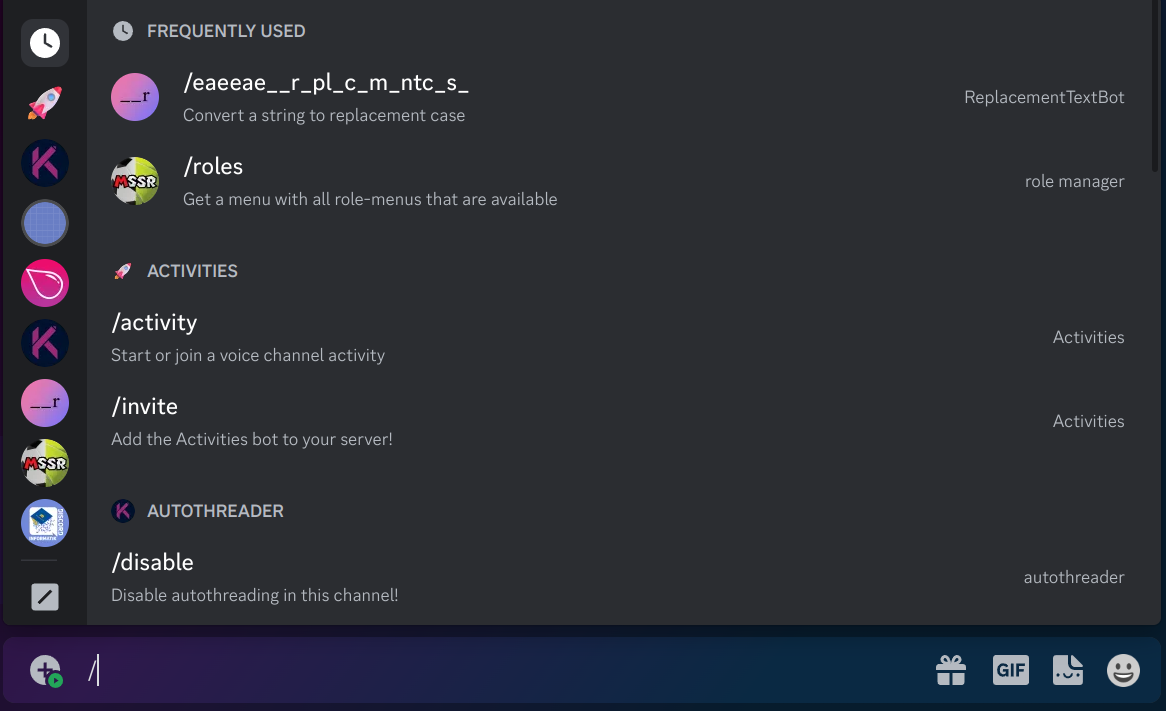
\includegraphics[height=0.7\textheight]{command_overview.png}
		\caption{Übersicht aller verfügbaren Bots und Commands auf diesem Server.}
	\end{figure}
\end{frame}


\begin{frame}{Ausführung und Antwort}
	\begin{figure}
		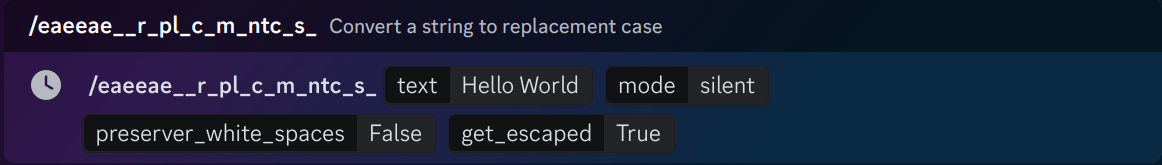
\includegraphics[width=.85\textwidth]{command_filled.png}
		\caption{Ausfüllen aller Parameter des Commands\furl{https://github.com/nonchris/IOEAEEAE\_\_d\_SC\_RD-r\_PL\_C\_M\_NT-c\_S\_}}
	\end{figure}
	\begin{figure}
		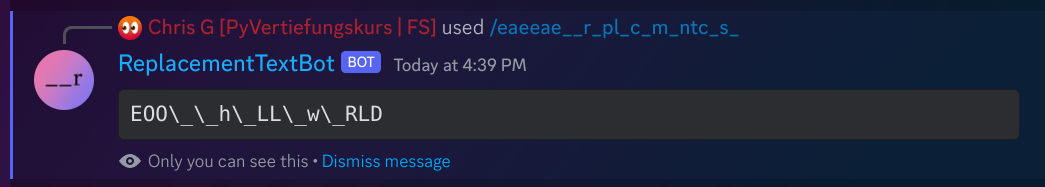
\includegraphics[width=.85\textwidth]{command_delivered.png}
		\caption{Die Anwtort ist eine nur für die ausführende Person sichtbare Nachricht.}
	\end{figure}
\end{frame}

% TODO: code beispiel


\begin{frame}[fragile]{Slash Commands}
	\begin{lstlisting}[language=pytiny]
from typing import Literal, Optional
import discord
from discord import app_commands

# use @app_commands.command instead if command is in Cog (fn must then also take self!)
@bot.tree.command(name="eaeeae__r_pl_c_m_ntc_s_", description="Convert to replacement case")
async def replacement_case_command(interaction: discord.Interaction, text: str,
        mode: Literal["silent", "loud"] | None, get_escaped: bool = False):
    """ Convert text from sARCASTIC_cASE to EAEEAE__r_PL_C_M_NTc_S_ """

    replacement_text = EAEEAE__r_PL_C_M_NTc_S_(text, eAE___SC_P_=True)

    if get_escaped:
        replacement_text = f"```{replacement_text}```"

    await interaction.response.send_message(replacement_text, ephemeral=mode == "silent")
	\end{lstlisting}
\end{frame}

% TODO: tasks


\begin{frame}[fragile]{Weitere Commands}
	\begin{itemize}
		\item \tb{ContextMenu}\furl{https://discordpy.readthedocs.io/en/stable/interactions/api.html\#contextmenu}\footnote{Beispiel aus \texttt{\_\_init\_\_} eins Cogs entnommen.}:\pause
		\item[] Fügt die Option hinzu, eine Aktion über das \tb{Kontext}-Menü von Discord auszulösen.
		\begin{lstlisting}[language=pytiny]
self.ctx_replacement = app_commands.ContextMenu(
    name='EAEEAE__r_PL_C_M_NTc_S_',
    callback=self.replacement_case_context,  # signature: (discord.Interaction, discord.Message)
)
self.bot.tree.add_command(self.ctx_replacement)	
		\end{lstlisting}

		
	\begin{figure}
		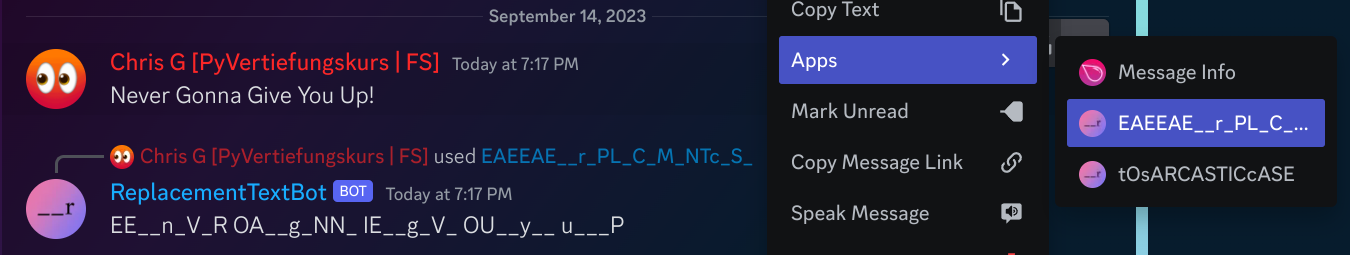
\includegraphics[height=.2\textheight]{command_context.png}
	\end{figure}
	
	\item Hinweis: Der \pp{tree} ist der \tb{zentrale} Ort für die Verwaltung von App Commands.
	
	\pause
	
	\item[] Dieses Objekt muss zum Start des Bots an alle Guilds \tb{gepushed} werden\footnote{Beispiel: \url{https://github.com/nonchris/discord-bot/blob/7ea672f499e7992a0e2d6076a419e43548f31f56/src/discord_bot/main.py\#L87}}.
		
	\end{itemize}
\end{frame}


\begin{frame}{Discord.py: Buttons \& Drowdown}
	\begin{itemize}
		\item Discord bietet Bots die Option \tb{Buttons}\furl{https://discordpy.readthedocs.io/en/latest/interactions/api.html\#id1}\furl{https://github.com/Rapptz/discord.py/blob/master/examples/views/dynamic\_counter.py} und \tb{Select}-Menus\furl{https://discordpy.readthedocs.io/en/latest/interactions/api.html?\#select-menus}\furl{https://github.com/Rapptz/discord.py/blob/master/examples/views/dropdown.py}.
		\item[] Diese können einer Nachricht angehängt werden.
		
		\pause
		
		\item Die Elemente verhalten sich \tb{analog} zu klassischen UI-Elementen:
		
		\pause
		
		\item[] \begin{itemize}
			\item Jedes \tb{erbt} von \pp{discord.ui.View}.
			
			\pause
			
			\item Jedes Element \tb{implementiert} eine \pp{callback}-Funktion, welche bei Press oder Auswahl ausgelöst wird.
		\end{itemize}
		
		\pause
		
		\item Pro versandtem View existiert \tb{eine} Instanz des Buttons bzw. DropDowns. Dieses kann u.A. weiteren \tb{individuellen} Kontext halten und weitere Methoden definieren.
		
		\pause
		
		\item Wird der Bot \tb{neugestartet}, sind alle vorherigen UIs nicht mehr funktionsfähig.
		
	\end{itemize}
\end{frame}


\begin{frame}[fragile]{Tasks}
	\begin{itemize}
		\item Alle bisherigen Funktionalitäten erfordern eine explizite Interaktion oder ein bestimmtes Event.
		
		\pause
		
		\item Für \tb{regelmäßig} auszuführende Aufgaben bietet Discord.py \tb{Tasks}\footnote{Diese liegen in \texttt{discord.ext.tasks}: \furl{https://discordpy.readthedocs.io/en/stable/ext/tasks/index.html}}.
		
		\pause
		
		\item Tasks werden \tb{gescheduled} und laufen dann in festen \tb{Zyklen} ab.
		
		\pause
		
		\item Tasks laufen unabhängig eines \pp{Guild}- / \pp{Message}-Kontextes.
		\item[] Daher müssen Informationen wie \pp{Guild}, etc. erst aus dem \pp{Bot} geholt werden\furl{https://discordpy.readthedocs.io/en/stable/ext/commands/api.html\#discord.ext.commands.Bot.get_guild}.
	\end{itemize}
	
	\pause
	
	\begin{lstlisting}[language=pytiny]
@tasks.loop(seconds=60)  # task runs every 60 seconds
async def my_background_task(self):      # this task is defined in bot istself, so self is the bot
    channel = self.get_channel(1234567)  # channel ID goes here
    self.counter += 1
    await channel.send(self.counter)
	\end{lstlisting}
	
\end{frame}


\begin{frame}[fragile]{Embeds}
	\begin{itemize}
		\item Discord bietet Bots die Möglichkeit, \tb{Nachrichten} als \pp{Embed}\furl{https://discordpy.readthedocs.io/en/stable/api.html\#embed} \tb{formatiert} zu versenden.
		
		\pause
		
		\item Diese biteten eine Reihe Formatierungs- und Strukturierungsoptionen.
		
		\pause
		
		\item Embeds werden einer Nachricht z.B. bei \pp{.send()} \tb{angehängt}.
		\item[] Sie dürfen mehr Text als normale Nachrichten enthalten.
		
		\pause
		
		\item Die \tb{Limits} für Embeds können hier\furl{https://discord.com/developers/docs/resources/channel\#embed-object-embed-limits} eingesehen werden.
	\end{itemize}
	
\end{frame}


\begin{frame}[fragile]{Beispiel Embed}

	
		\begin{figure}
			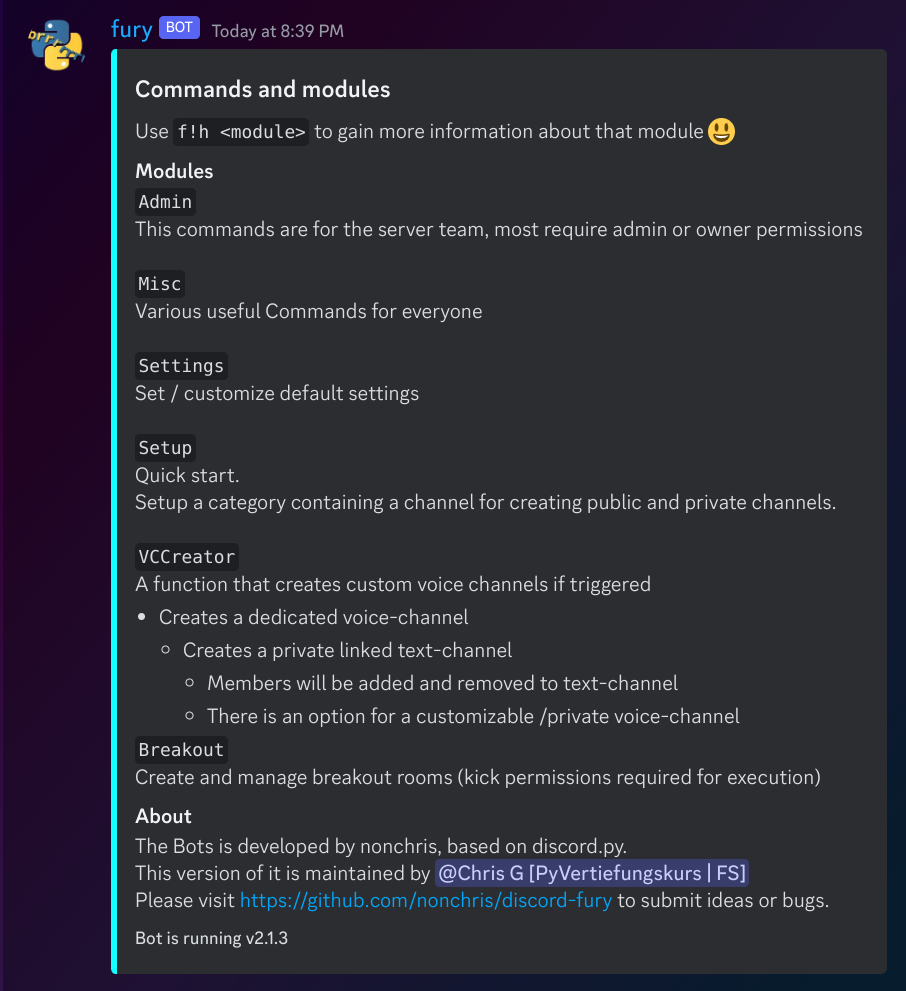
\includegraphics[height=.7\textheight]{embed.png}
			\caption{Help Command von fury: \url{https://github.com/nonchris/discord-fury/}}
		\end{figure}

\end{frame}


\begin{frame}{Hinweise \& Best Practices}
	\begin{itemize}
		\item Hinzufügen/ Entfernen von z.B. Rollen: \pp{set}-Operationen!
		
		\pause
		
		\item Nutz vernünftiges \tb{Logging}, da das Programm viel im Hintergrund laufen wird!
		
		\pause
		
		\item Das \tb{Context}-Objekt heißt immer \pp{ctx}.
		
		\pause
		
		\item Die \pp{.ext} Module werden als \pp{from discord.ext import commands} bzw. \pp{tasks} eingebunden.
		
		\pause
		
		\item Discord.py bietet einiges an \tb{utility}-Functions, welche das Leben wirklich einfacher machen\furl{https://discordpy.readthedocs.io/en/stable/api.html\#utility-functions}.
		\item Hat man einen Discord Bot, welcher Interactions anbietet und quasi regelmäßig genutzt wird, erhält man das coole (neue) \tb{Developer-Badge}.
		
		\pause
		
		\item \tb{TOKENS} \pause werden \pause \tb{NIEMALS} \pause in \pause den \pause \tb{CODE \pause EIN\pause GE\pause FÜGT\pause!} 
	\end{itemize}
\end{frame}


\begin{frame}{Sources und Samples}
	\begin{itemize}
		\item \tb{API-Reference}: \url{https://discordpy.readthedocs.io/en/stable/api.html}
		
		\item Discord.py \tb{Examples}:\\
		\url{https://github.com/Rapptz/discord.py/tree/master/examples}
		
		\item Ein ziemlich gutes \tb{Template}:\\
		\url{https://github.com/nonchris/discord-bot}
		
		\item \tb{Welcome} Dialogue (Info Bonn):\\
		\url{https://github.com/Info-Bonn/welcome-dialogue/} 
		
		\item Role \tb{Selection}:\\
		\url{https://github.com/nonchris/discord-role-selection}
		
		\item The \tb{future} of code:\\
		\url{https://github.com/nonchris/IOEAEEAE__d_SC_RD-r_PL_C_M_NT-c_S_}
		
	\end{itemize}
\end{frame}


\framecardfragen



\section{Deployment}

% note @ myself:
% \pause is very useful
% \pp & \tb is used for highlighting

\begin{frame}[fragile]{Wer ist Niklas Steffen?}
	\tb{Beruf und Studium:}
	\begin{itemize}
		\item seit 2018: \tb{Informatik Student} an der Universität Bonn
		\item \pause 2017-2021: \tb{Systemadministrator} für Mittelständige Unternehmen
		\item \pause seit 2021: NixOS \tb{Contributor \& Maintainer}
		\item \pause seit 2021: \tb{Head of IT} für die Firma AFM (im sozialem Bereich tätig)
	\end{itemize}
	
	\tb{Interessen:} \nll{Für die Veranstaltung relevante Interessen}
	\begin{itemize}
		\item Server und \tb{Netzwerkinfrastruktur}
		\item System Verwaltung und \tb{Automatisierung}
		\item Rennräder
	\end{itemize}
\end{frame}

\begin{frame}[fragile]{Disclaimer}
	\begin{itemize}
		\nll{ich kann nur einen groben Überblick geben}
		\item \pause \tb{Halbwissen} ist vor allem bei diesem Thema sehr \tb{gefährlich}! Do your own research!
		\item \pause Dieser Vortrag basiert zu Teilen auf meine \tb{Erfahrungen} und persönlichen \tb{Meinungen}. Ich gebe mir Mühe, diese als solche zu kennzeichnen.
	\end{itemize}
\end{frame}

\begin{frame}[fragile]{Was verstehen wir unter Deployment?}
	\tb{Cambridge Dictionary\furl{https://dictionary.cambridge.org/de/worterbuch/englisch/deployment}:}
	\begin{itemize}
		\item the \tb{use} of \tb{something} or someone in an \tb{effective} way
		\item the movement of soldiers or equipment to a place where they \tb{can be used} when they are \tb{needed}
	\end{itemize}
	\tb{Niklas Steffen (im Kontext von Softwareentwicklung):}
	\begin{itemize}
		\item Software wird auf einem Server \tb{deployed}, damit sie von den Nutzern \tb{verwendet} werden kann
		\item Deployment ist die \tb{letzte Phase} des Softwareentwicklungsprozesses und ein Teil von \tb{DevOps} \nll{Fragt nach, ob jemand weiß was DevOps ist}
		\item Ohne Deployment bleibt die Software \tb{ungenutzt}
	\end{itemize}
\end{frame}

\begin{frame}[fragile]{Was ist Deployment?}
	\tb{Wieso ist Deployment auch für Entwickler wichtig?}
	\begin{itemize}
		\item \tb{Entwicklungsumgebungen} sind nicht immer identisch zu \tb{Produktivumgebung} (bspw. andere \tb{Betriebssysteme}, Software \tb{Versionen} oder \tb{Hardware})
		\item Wenn \tb{Entwickler} in den Deployment Prozess \tb{involviert} sind, können \tb{Fehler vermieden} werden, die sich erst im Deployment Prozess zeigen würden
		\item \tb{Meinung:} Das \tb{Verständnis} des Deployment Prozesses hilft Entwicklern dabei, besser auf die Produktivumgebung angepasste Software zu schreiben
		\item \tb{Meinung:} Die \tb{Kommunikation} zwischen Entwicklern und Systemadministratoren sorgt für einen \tb{reibungslosen} Deployment Prozess \nll{Anekdote was ich an der Zusammenarbeit mit Chris schätze}
	\end{itemize}
\end{frame}

\begin{frame}[fragile]{Was ist Deployment?}
	\tb{Was möchte ich heute vermitteln?}
	\begin{itemize}
		\item \pause \tb{Zusammenhang} zwischen Softwareentwicklung und Deployment (DevOps)
		\item \pause Unterschiede zwischen \tb{Client} und \tb{Server} Anwendungen
		\item \pause Kathegorisierung von Anwendungen (\tb{Anforungsanalyse})
		\item \pause Unterschiede zwischen \tb{Cloud} und \tb{on premise} Deployment
	\end{itemize}
\end{frame}

\begin{frame}[fragile]{Kathegorisierung von Anwendungen}
	\tb{Echtzeit Anwendungen vs. Nicht Echtzeit Anwendungen}
	\begin{itemize}
		\item \pause \tb{Gameserver} \pause (Echtzeit Anwendung)
		\item \pause \tb{Voice over IP} \pause (Echtzeit Anwendung)
		\item \pause \tb{Discord Bot} \pause (Interaktive Anwendung ohne Echtzeit Anforderungen)
		\item \pause \tb{Git Server} \pause (Interaktive Anwendung ohne Echtzeit Anforderungen)
		\item \pause \tb{Transcoding Server} \pause (Batch Anwendung ohne Echtzeit Anforderungen)
		\item \pause \tb{Transcoding Server für Live Streams} \pause (Echtzeit Anwendung)
		\item \pause \tb{Compiler} \pause (Batch Anwendung ohne Echtzeit Anforderungen)
		\item \pause \tb{Webserver} \pause (Hängt von der Anwendung ab)
	\end{itemize}
\end{frame}

\begin{frame}[fragile]{Kathegorisierung von Anwendungen}
	\tb{Wo wird die Anwendung ausgeführt?}
	\begin{itemize}
		\item \pause auf einem \tb{Server}
		\item \pause auf einem \tb{Client} System
	\end{itemize}
\end{frame}

\begin{frame}[fragile]{Client Anwendungen}
	\begin{itemize}
		\item \pause Client Anwendungen werden auf dem System des Nutzers \tb{ausgeführt} und durch den Nutzer \tb{installiert}
		\item \pause Anwendungen müssen an Nutzer \tb{verteilt} werden (bspw. über den Browser, über einen App Store, Paketmanager, etc.)
		\item \pause Dies geschieht häufig über CI Pipelines, die die Anwendung \tb{bauen} und dann zum Download \tb{bereitstellen}
		\item \pause Unter Linux sind die \tb{Maintainer} der Repositorys für die Bereitstellung der Anwendungen \tb{verantwortlich}
		\item \pause Im Python Umfeld ist die \tb{Verteilung} über PyPI üblich
	\end{itemize}
	\tb{Das saubere Paketieren von Anwendungen ist wichtig!} \nll{Wichtig weil die Verteilung und damit auch die Nutzung der Anwendung davon abhängt.}
\end{frame}

\begin{frame}[fragile]{Server Anwendungen}
	\tb{Betriebssystem?}
	\begin{itemize}
		\item \pause Deployment findet fast immer auf \tb{Linux} Systemen statt
	\end{itemize}
	\tb{Wo steht der Server?}
	\begin{itemize}
		\item \pause In der \tb{Cloud}
		\item \pause \tb{On premise} (Hardware wird innerhalb der eigenen Räumlichkeiten betrieben)
	\end{itemize}
\end{frame}

\begin{frame}[fragile]{die Cloud}
	\nll{Cloud ist ein Wort, mit welchem Unternehmen gerne Bingo spielen.}
	\nll{Infrastruktur as a Service, welche in einem Rechenzentrum betrieben wird}
	\nll{Wir beschränken uns auf VPS / Root Server}
	\begin{figure}
		
\includegraphics[width=0.4\textwidth]{images/thereisnocloud-sticker-74mm-blackwhite.en.pdf}
		\caption{https://fsfe.org/contribute/spreadtheword.en.html}
	\end{figure}
\end{frame}

\begin{frame}[fragile]{die Cloud}
	\nll{Erwähnen, dass Kosten einer der wichtigsten Punkte  bezüglich der Auswahl unserer Plattform sind}
	\nll{Erwähnen, dass ich mich gerade auf die Zielgruppe Vertiefungskurs Teilnehmer beziehe}
	\tb{Kosten}
	\begin{itemize}
		\item \pause Abhängig von \tb{CPU} Reccourcen, \tb{RAM}, \tb{Speicher}, \tb{Netzwerk} Anbindung, etc.
		\item \pause Häufig ohne feste Laufzeit (Abrechnung pro Stunde)
		\item \pause Oft zusätzliche Kosten bspw. für \tb{Traffic, Backups, Snapshots}, etc.
	\end{itemize}
	\tb{Nachteile}
	\begin{itemize}
		\item \pause Reccourcen sind vergleichsweise \tb{teuer} \nll{Wieso sind die Preise teurer? Was bekommt man dafür?}
		\item \pause Preise sind \tb{nicht} immer \tb{transparent} (bspw. bei AWS, Azure, Google Cloud) \nll{Wieso sind Preise nicht transparent?}
	\end{itemize}
\end{frame}

\begin{frame}[fragile]{die Cloud}
	\tb{Wann bietet sich Cloud Deployment an?}\\
	\begin{itemize}
		\item \pause Bei Projekten bei denen eine hohe \tb{Verfügbarkeit} und schnelle \tb{Netzwerk Anbindung} wichtig sind
		\item \pause Bei Projekten, mit \tb{geringen Anforderungen} an die Hardware
		\item \pause Bei Projekten, bei denen sich die Hardware Anforderungen \tb{häufig ändern}
		\item \pause Bei Projekten, die nur für eine \tb{begrenzte Zeit} laufen sollen
		\item \pause Bei Projekten, bei denen die Hardware Anforderungen \tb{nicht bekannt} sind \nll{Wieso ist das ein Vorteil?}
	\end{itemize}
\end{frame}

\begin{frame}[fragile]{on premise}
	\tb{Einmalige Kosten}
	\begin{itemize}
		\item \pause Hardware (Server, Netzwerkinfrastruktur, USV's, etc.)
		\item \pause Lizenzen
		\item \pause Backup Festplatten
	\end{itemize}
	
	\tb{laufende Kosten}
	\begin{itemize}
		\item \pause Strom
		\item \pause Internet Anbindung
		\item \pause Offsite Backups (wenn in der Cloud)
	\end{itemize}
\end{frame}

\begin{frame}[fragile]{on premise}
	\nll{Parrallelen zum Cloud Deployment ziehen. Sprechen von privaten Projekten}
	\tb{Nachteile}
	\begin{itemize}
		\item \pause Hohe \tb{einmalige} Kosten
		\item \pause Hoher \tb{Wartungsaufwand} (Hardware Ausfälle, Reinigung, etc.)
		\item \pause \tb{Unflexibel} (Hardware kann nicht einfach gekündigt oder verändert werden)
		\item \pause \tb{Wärme und Lärm} (kann vermieden werden)
		\item \pause Bietet sich nicht für jede \tb{Wohnsituation} an
		\item \pause Hoher \tb{Aufwand} für die Einrichtung (da nicht rein in Software)
		\item \pause \tb{Langsamere} Internet Anbindung (im Vergleich zu Cloud Anbietern)
		\item \pause \tb{Sicherheits Risiken} können oft nicht gut eingeschätzt werden
		\nll{Darauf eingehen, dass die meisten dieser Nachteile behoben werden können, aber zusätzliches Wissen und Aufwand erfordern. Erklären wieso Security Risiken nicht gut eingeschätzt werden können und welche Maßnahmen man ergreifen kann}
	\end{itemize}
\end{frame}

\begin{frame}[fragile]{on premise}
	\tb{Wann bietet sich on premise Deployment an?}
	\begin{itemize}
		\item \pause Bei bereits \tb{vorhandener} Hardware
		\item \pause Bei \tb{bekannten} Hardware Anforderungen
		\item \pause Bei Projekten die \tb{langfristig} laufen sollen
		\item \pause Bei einem \tb{hohen} Ressourcen Bedarf
		\item \pause Wenn besondere Hardware benötigt wird (bspw. \tb{Grafikkarten})
		\item \pause Bei Projekten, welche \tb{nicht public facing} sein müssen
		\item \pause Wenn die Nutzer sich im \tb{selben Netzwerk} befinden
	\end{itemize}
\end{frame}

\begin{frame}[fragile]{Software Stack (für Interessierte)}
	\begin{itemize}
		\item \pause \tb{Virtualisierung} (KVM, ESXI, Hyper-V, etc.)
		\item \pause \tb{SSH} (OpenSSH, Dropbear, etc.)
		\item \pause \tb{Automatisierung und Konfigurationsmanagement} (Ansible, Cloud Init, etc.)
		\item \pause Cloud API's (AWS, Azure, Google Cloud, etc.) durch bspw. \tb{Terraform}
		\item \pause \tb{Monitoring} (Prometheus, Grafana, Zabbix, etc.)
		\item \pause \tb{Logging} (ELK Stack, Graylog, etc.)
		\item \pause \tb{Backups} (Borg, Restic, etc.)
		\item \pause \tb{Firewall} (iptables, nftables, etc.)
		\item \pause \tb{Deep Packet Inspection} (Suricata, Snort, etc.)
		\item \pause \tb{Git} Server mit CI Pipeline
		\item \pause \tb{Container} und Container \tb{Orchestrierung} (Docker, Kubernetes, etc.)
		\item \pause \tb{Systemd}
		\item \pause \tb{Reverse Proxy} (Nginx, HA-Proxy, Traefik, etc.)
	\end{itemize}
\end{frame}

\begin{frame}[fragile]{Docker}
	\tb{Nachteile:}
	\begin{itemize}
		\item \pause Sicherheits Updates werden erschwert (Images müssen neu gebaut werden)
		\item \pause Sehr viele Images weisen \tb{Sicherheitslücken} auf
		\item \pause Vertrauen in den Image Ersteller ist wichtig
		\item \pause Häufig werden \tb{veraltete} Images verwendet
		\item \pause Häufig werden Anwendungen innerhalb des Containers \tb{als root} ausgeführt \nll{Wieso ist das ein Problem?}
		\item \pause Dockerfiles und Entrypoints können \tb{komplex} werden
		\item \pause Angreifer können Kontrolle über den Container erlangen
		\item \pause Über Bind Mounts und Privileges ist auch ein \tb{Zugriff} auf das \tb{Host System} möglich
	\end{itemize}
\end{frame}

\begin{frame}[fragile]{Docker}
	\tb{Fazit:}
	\begin{itemize}
		\item \pause Um Docker \tb{sicher} zu betreiben, ist \tb{Wissen} über Linux \tb{Sicherheit} notwendig.
		\item \pause Docker ist keine \tb{Sicherheitslösung} und sollte auch nicht als solche verwendet werden.
		\item \pause Container nutzen \tb{Kernel Namespaces} und \tb{Cgroups}. Die Isolierung einer Anwendung wäre auch ohne Docker möglich.
	\end{itemize}
\end{frame}

\begin{frame}[fragile]{Beispiele}
	\tb{welcome dialogue (discord bot)}\furl{https://github.com/Info-Bonn/welcome-dialogue}
	\begin{itemize}
		\item \pause \tb{Interaktive} Anwendung ohne Echtzeit Anforderungen (Verzögerungen von mehreren Sekunden haben \tb{keinen} Einfluss auf die Nutzbarkeit)
		\item \pause Sehr \tb{geringe Anforderungen} an die Hardware
		\item \pause \tb{Verfügbarkeit} wichtig, damit neue Mitglieder dem Discord Server beitreten können
		\item \pause Aufgrund der geringen Anforderungen an die Hardware, ist ein \tb{Cloud} Deployment hier sehr \tb{günstig}.
		\item \pause Mit den sehr geringen Kosten \tb{erkaufen} wir uns eine hohe Verfügbarkeit
		\item \pause Wir sind \tb{unabhängig} von unserer Internet Anbindung zu Hause
	\end{itemize}
\end{frame}

\begin{frame}[fragile]{Beispiele}
	\tb{Whisper API}
	\begin{itemize}
		\item \pause \tb{Batch} Anwendung (Jobs werden nacheinander abgearbeitet)
		\item \pause \tb{Interaktiv} (Nutzer warten auf ein Ergebnis)
		\item \pause Damit die Anwendung \tb{sinvoll} genutzt werden kann, müssen die Jobs schnell abgearbeitet werden
		\item \pause Um die API enorm zu beschleunigen, brauchen wir eine \tb{Grafikarte}, die das Modell ausführen kann
		\item \pause \tb{Grafikkarten} kosten in der Cloud mehrere tausend Euro pro Monat
		\item \pause On premise Deployment ist hier die \tb{einzige Option}
		\item \pause Um nur \tb{berechtigte Zugriffe} zu erlauben, setzten wir \tb{Keycloak} als \tb{Idendity Provider} ein
		\item \pause Reverse Proxy (\tb{Nginx}) leitet \tb{berechtigte} Anfragen an unseren GPU Server weiter
	\end{itemize}
\end{frame}

\begin{frame}[fragile]{Beispiele}
	\tb{Whisper API}\furl{https://github.com/MayNiklas/whisper_api}
	\begin{figure}
		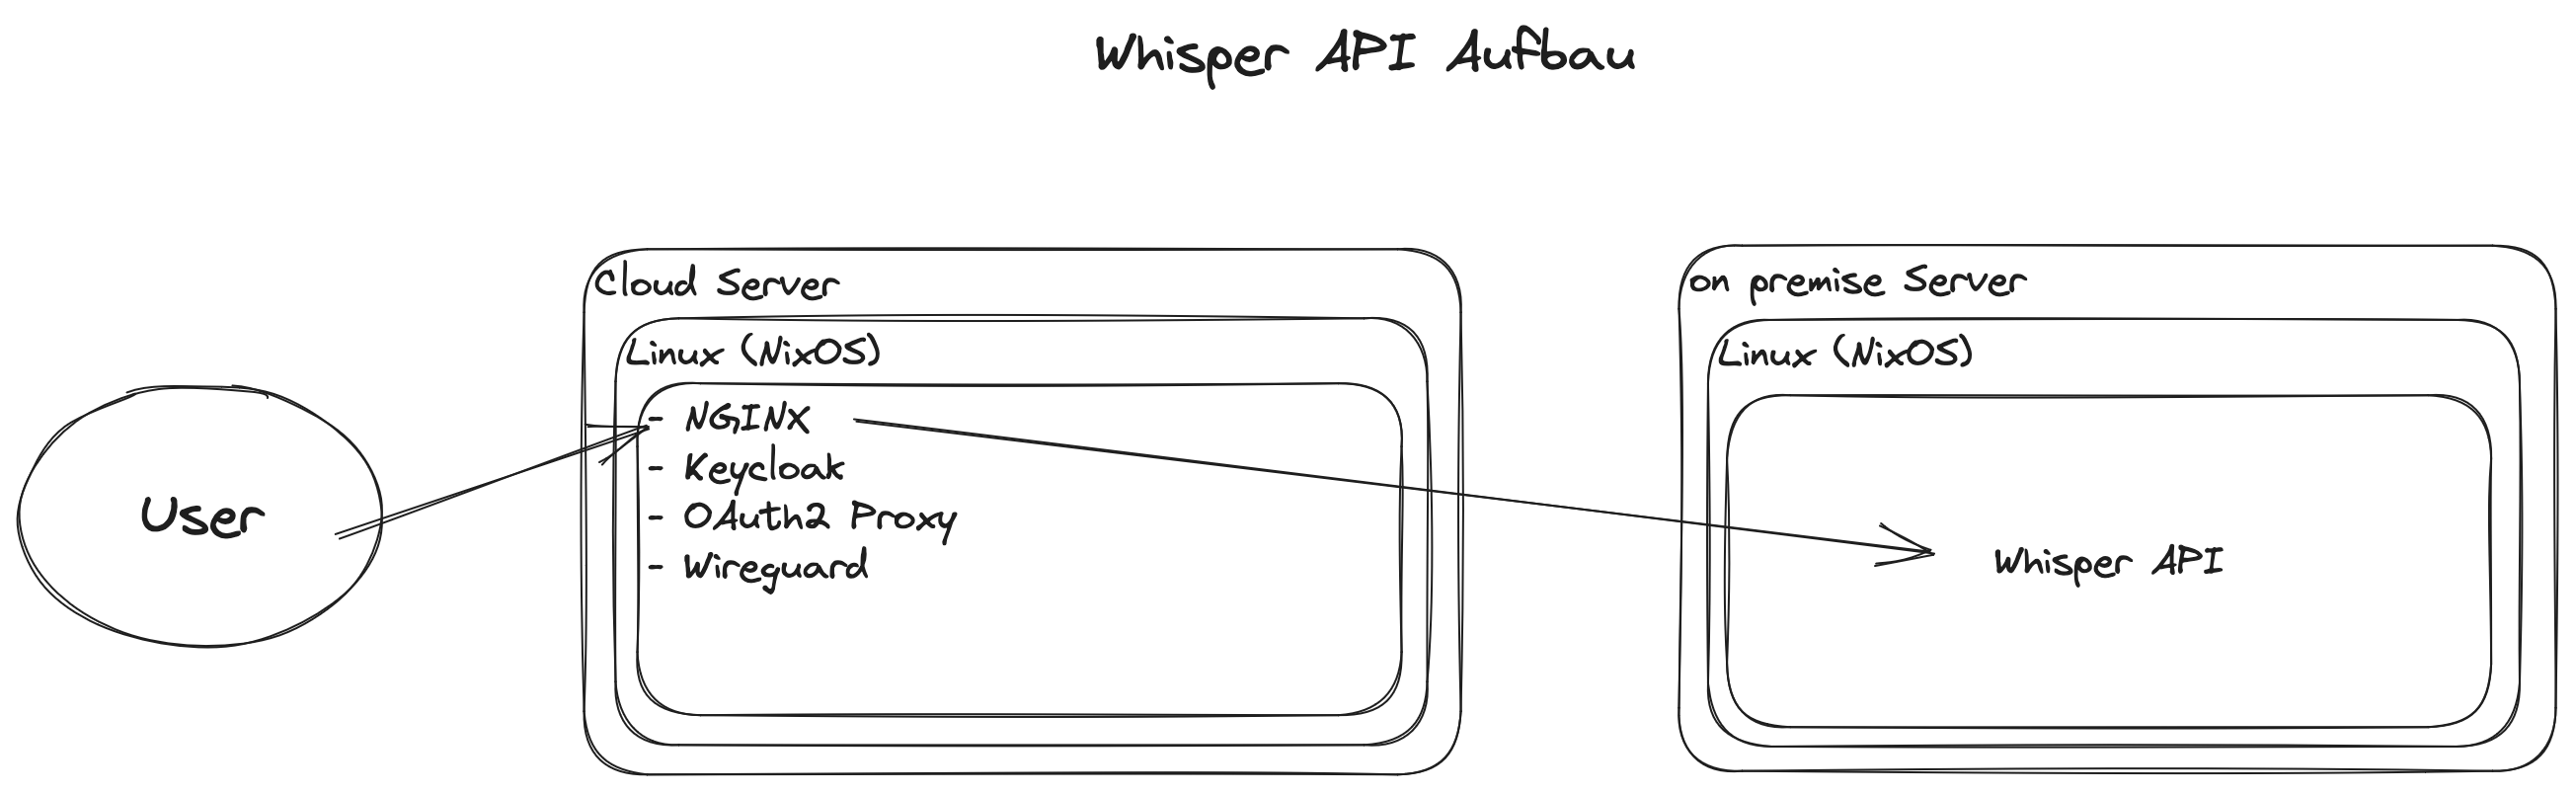
\includegraphics[width=1\textwidth]{images/Whisper-api.png}
	\end{figure}
\end{frame}

\begin{frame}[fragile]{Beispiele}
	\tb{Minecraft Server}
	\begin{itemize}
		\item \pause \tb{Echtzeit} Anwendung (wenn Server zu langsam ist, \tb{laggt} es für die Spieler)
		\item \pause Minecraft Server sind sehr \tb{CPU \& RAM} intensiv
		\item \pause Cloud Deployment wird schnell \tb{teuer}
		\item \pause On premise Deployment ist eine Option, die viel \tb{Geld sparen} kann
		\item \pause Vor und Nachteile müssen \tb{abgewogen} werden
	\end{itemize}
\end{frame}

\begin{frame}[fragile]{Erste Projekte}
	\tb{Eigenschaften:}
	\begin{itemize}
		\item \pause \tb{nicht} public facing
		\item \pause \tb{geringe} Anforderungen an die Hardware
		\item \pause ohne Abhängigkeiten zu \tb{anderen Services}
		\item \pause ohne Abhängigkeiten zu \tb{anderen Systemen}
	\end{itemize}
	\pause\tb{Beispiele:}
	\begin{itemize}
		\item \pause \tb{Discord Bot}
		\item \pause \tb{Webserver} der nur lokal (oder via VPN) erreichbar ist
		\item \pause Bspw. ein \tb{Web Frontend} für ein anderes Projekt
		\item \pause Es bieten sich auch \tb{fertige Projekte} an
	\end{itemize}
\end{frame}

\begin{frame}[fragile]{Hardware Optionen}
	Hardware beeinflusst:
	\begin{itemize}
		\item \pause \tb{Kosten} (einmalig und laufend)
		\item \pause \tb{Leistung} (CPU, RAM, Speicher, Netzwerk, etc.)
		\item \pause \tb{Stromverbrauch}
		\item \pause \tb{Lärm und Wärme}
		\item \pause \tb{Upgrade Möglichkeiten}
		\item \pause \tb{Verfügbarkeit} (wie viel Redundanz?)
	\end{itemize}
\end{frame}

\begin{frame}[fragile]{Hardware Optionen}
	\begin{itemize}
		\item \pause Raspberry Pi
		\item \pause Intel NUC
		\item \pause Mini PC (bspw. Lenovo ThinkCentre)
		\item \pause alter PC oder Laptop
		\item \pause Gebrauchte Server Hardware
	\end{itemize}
	Hinweis: diese Auflistung macht ohne den gesprochenen Kontext keinen Sinn.\\
	Ich rate explizit von vielen Optionen ab!
\end{frame}

\begin{frame}[fragile]{Kontakt}
	\begin{itemize}
		\item GitHub: @MayNiklas \furl{https://github.com/MayNiklas}
		\item Matrix: @mayniklas:matrix.lounge.rocks
		\item Discord: @mayniklas
		\item E-Mail: info@niklas-steffen.de
	\end{itemize}
\end{frame}


\framecardfragen

\silentsection{Honerable Mentions}
\subsection{Stoff für mindestens eine weitere Woche}


\begin{frame}[fragile]{Honerable Mentions I}
	\begin{itemize}
		\item Abstarct Baseclasses\furl{https://docs.python.org/3/library/collections.abc.html\#collections-abstract-base-classes}: Eigene typehint-bare \tb{Typen} erstellen.
		
		\item Beautiful Soup\furl{https://www.crummy.com/software/BeautifulSoup/bs4/doc/}: \tb{HTML} und XML parsen.
		
		\item Collections\furl{https://docs.python.org/3/library/collections.html} und insb. das \tb{defaultdict}.
		
		\item deepcopy\furl{https://docs.python.org/3/library/copy.html\#copy.deepcopy}: \tb{Vollständige} Kopien eines Objektes erzeugen.
		
		\item inspect\furl{https://docs.python.org/3/library/inspect.html\#module-inspect}: \tb{Funktionssiganturen} und anderen Dinge zur Laufzeit analysieren.
		
		\item os\furl{https://docs.python.org/3/library/os.html\#module-os}: Interaktion mit dem Datei- und \tb{Betriebssystem}.
		
	\end{itemize}
\end{frame}


\begin{frame}[fragile]{Honerable Mentions II - Libraries mit P}
	\begin{itemize}

		
		\item Pathlib\furl{https://docs.python.org/3/library/pathlib.html\#pure-paths}: \tb{Dateipfade in Python}
		
		\item Pillow\furl{https://pypi.org/project/Pillow/} \tb{Bilder} einlesen und verarbeiten.
		
		\item pynput\furl{https://pypi.org/project/pynput/}: \tb{Tastatur} und Maus simulieren.
		
		\item PyPDF2\furl{https://pypi.org/project/PyPDF2/}: \tb{PDFs} einlesen und bearbeiten.
		
		\item python-telegram-bot\furl{https://pypi.org/project/python-telegram-bot/}: \tb{Telegram} Bots
		
	\end{itemize}
\end{frame}


\begin{frame}[fragile]{Honerable Mentions III}
	\begin{itemize}
		
		
		\item qrcode\furl{https://pypi.org/project/qrcode/}: \tb{QR-Codes} erstellen.
		
		\item re\furl{https://docs.python.org/3/library/re.html}: \tb{RegEx} in Python.
		
		\item Selenium\furl{https://pypi.org/project/selenium/}: Einen \tb{Browser} mit Python steuern.
		
		\item subprocess\furl{https://docs.python.org/3/library/subprocess.html}: \tb{Command Line} Befehle aus Python heraus ausführen.
		
		\item tempfile\furl{https://docs.python.org/3/library/tempfile.html}: \tb{Temporäre} (benannte) Dateien erstellen.
	\end{itemize}
\end{frame}


\begin{frame}{Evaluation und Sticker}
	\begin{figure}
		\begin{center}
			
\includegraphics[height=.66\textheight]{survey.png}
			\caption{\url{https://limesurvey.informatik.uni-bonn.de/index.php/627488?lang=de-informal}}
		\end{center}
	\end{figure}
\end{frame}

\framecardblue{
	\Utext{Vielen Dank, dass Du da warst!\\ -Chris}
}


\end{document}

